

Tuscarora provides a flexible deployment procedure in which modules depicted in \cref{Fig:Goal} can run in their own processes or several of these modules can be bundled to share a single process. 
In order to enable deployments on various platforms and 
to provide a common architecture for single process or multi-process setups, 
Tuscarora defines a communication module that translates calls between various layers. We colloquialy refer to this as the ``communication shim layer'' or just as ``shim''; 
A shim layer is required  between the applications and the patterns, between the patterns and the framework, and between the framework and waveforms as shown in \cref{fig:CommonShimLayerInterface}.

Tuscarora APIs are designed with function syntax(aka method calls) and named with message passing semantics.
The job of the shim layer is to translate a function call from within one layer to a function call on another layer, using asynchronous message passing between layers.
For example, a pattern makes a call to a shim layer object and the shim layer object calls the framework, which might be part of the same process space or might be running as a different process. For multi-process environments,
this shim layer should convert the function calls to messages or some other inter-process mechanism (such as pipes) and send them to the corresponding modules on the other layer.
Similarly, the shim layer parses and converts received messages back into function calls and invokes the corresponding functions on the receiving layer.

\begin{figure}[ht]
	\centering
	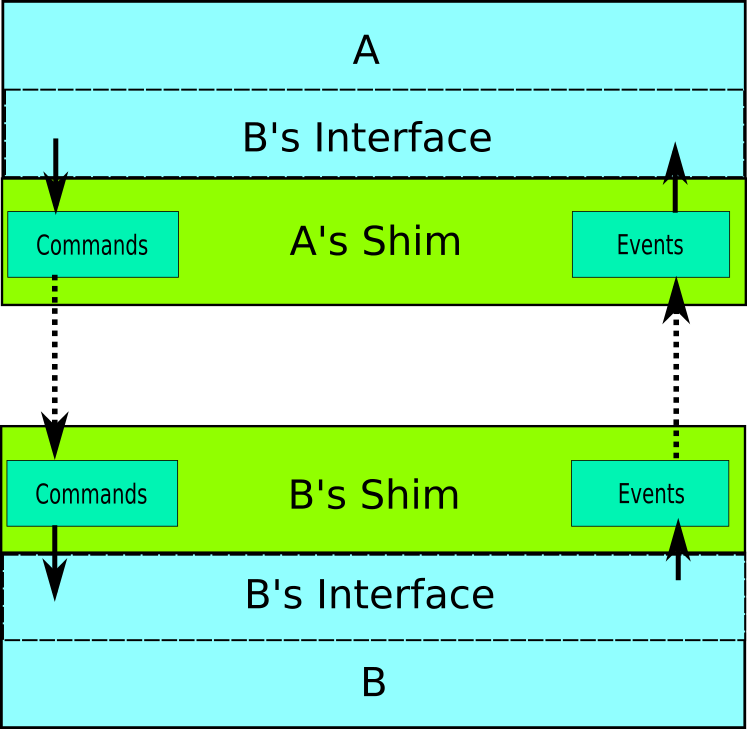
\includegraphics[width=0.3\linewidth]{figures/CommonShimLayerInterface}
	\caption{Generic example of Shims between Layer A and Layer B, where A is user of B}
	\label{fig:CommonShimLayerInterface}
\end{figure}


In a single-process environment, a shim layer can be implemented using one of the many different options available, such as synchronous blocking function call, asynchronous non-blocking function calls, messaging passing or signaling.
In general, the implementation of these shim layers can be platform-specific and when porting Tuscarora to a new platform at least some of the shim layer modules may need to be reimplemented.
Tuscarora interfaces are designed with `Commands' that are received by a module and `Events' that are invoked or sent from a module, i.e., Tuscarora interfaces are bidirectional. For example, consider two layers , A and B, as shown in \cref{fig:CommonShimLayerInterface}. 
If layer A wants to invoke a command on layer B, then a communication shim is need both on A's side to send out the Commands and to receive  B's Events. On B's side we need a shim to receive the commands and to send out the Events. 
However, sometimes (mostly in single process case), the shim on either A or B can be skipped, if they have a common shared memory location. 
The Shim on A's side should implement B's interfaces, both Commands and Events. 
That is A's shim translates from B's interface to some common agreed upon communication standard between A and B, and B's shim translates back this communication standard back to B's interface specification and invokes B.  Therefore A's shim looks like B to A.


Tuscarora package provides shim layers designed for the DCE environment as well as linux multi-process environments. 

\section{App-Pattern Shim Layer Modules}

Applications can be written towards the interface definitions of one or more patterns. 
Depending on the platform, the object implementing the interface could be the pattern itself or a pair of shim layers that pass the call to the intended pattern. \Cref{fig:AppPatternInterface} depicts setups for multi-process and single process environments. 

\begin{figure}[ht]
\centering
	  \begin{minipage}[b]{0.4\textwidth}
	    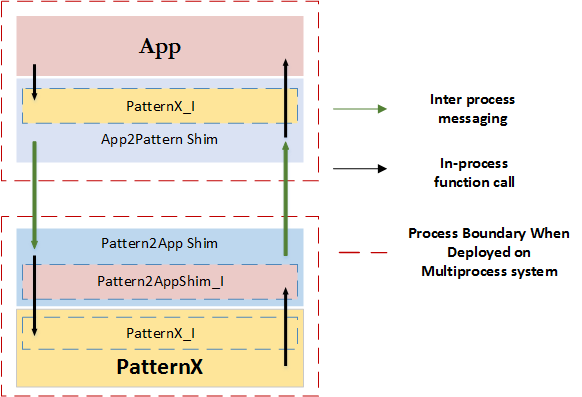
\includegraphics[width=\textwidth]{figures/App_Pattern_ShimArchitectureMP}
	    %\caption{multi process platform}
	    %\label{fig:AppPatternInterfaceMP}
	  \end{minipage}
	  \hspace{5mm}
	  \begin{minipage}[b]{0.4\textwidth}
	    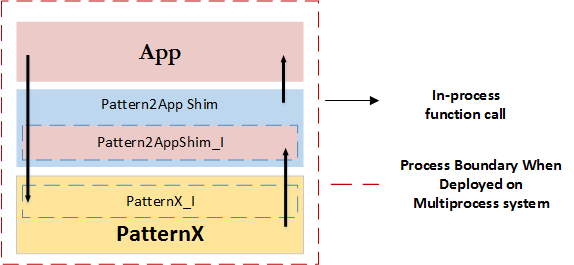
\includegraphics[width=\textwidth]{figures/App_Pattern_ShimArchitectureSP}
	    %\caption{single process platform}
		%\label{fig:AppPatternInterfaceSP}
	  \end{minipage}
\caption{App-Pattern interface for multi process and single process environments}
\label{fig:AppPatternInterface}
\end{figure}


\subsection{Multi process Shim Setup}

In multi process environments, \CPPClassName{App2PatternShim} and \CPPClassName{Pattern2AppShim} \CPPClassName{App2FWPShim} pair carry calls from each side of the process to the other side. Internally, these calls are converted to serialized messages on the sending side and carried over using a socket communication interface. Once received, the message is deserialized and the destination layer is called with the variables inside message. 

Tuscarora provides \CPPClassName{SocketCommunicatorClientBase} and the \CPPClassName{SocketCommunicatorServerBase} classes to automate server-client connection process, and \CPPClassName{GenericSerializer} and \CPPClassName{GenericDeSerializer} templated classes that help serialization and deserialization process for the shim classes. 


\CPPClassName{SocketCommunicator} library simply provides functions to send serialized buffers to the other side and on receiving event it directs read contents to a virtual \CPPFuncName{Deserialize} function implemented by the corresponding shims. 

A generic serializer object is simply constructed by listing the list of variable types and the corresponding variables and it creates a serialized buffer that contains copies of the variable values. Similarly, a generic de-serializer deserializes a variable sized buffer by copying its content to individually created variables in the order specified in its constructor. They also accepts pointers in which case the value of the preceding variable is assumed to be the size of the object pointed by the pointer. 


We'll elaborate this process with an example call to SendData from the \TuscConcept{FanOutFWP} application to \TuscConcept{FWP} pattern. 

\CPPClassName{App2FWPShim}'s \CPPFuncName{SendData} uses a GenericSerializer object to create a serialized buffer consisting of a calltype, and the function inputs, namely \CPPVarName{AppId\_t}, the variable sized message and a nonce that is used to identify the message between the app and the pattern. Then \CPPClassName{App2FWPShim} calls the \CPPFuncName{SendMsg2Server} function implemented by the base class, \CPPClassName{SocketCommunicatorClientBase}, to send the serialize message to the corresponding server.

Upon receiving the signal ,the message contents are read from the socket by \CPPClassName{FWP2AppShim}'s base class \CPPClassName{SocketCommunicatorClientBase} and \CPPFuncName{Deserialize} function of \CPPClassName{FWP2AppShim} is invoked. \CPPFuncName{Deserialize} function, first reads the calltype from the received buffer. Depending on the calltype, the rest of the buffer is deserialized into individual variables. In the case of the calltype being \CPPVarName{APP2FWP\_Call\_Send}, the rest of the buffer is deserialized into an \CPPVarName{AppId\_t}, a variable sized message and a nonce using a \CPPClassName{GenericDeSerializer}. Using these variables, the  \TuscConcept{FWP} pattern's \CPPFuncName{SendData} function is invoked. Hence, the call from \TuscConcept{FanOutFWP} to \TuscConcept{FWP} is completed. 


\subsection{Single process Shim Setup}

In single process setups, such as the ones DCE platform uses, \TuscConcept{App2PatternShim} disappears and the function calls directly invokes implementations in the \TuscConcept{PatternX} as depicted in \cref{fig:PatternFrameworkInterface}. \TuscConcept{Pattern2AppShim} only acts as a dispatcher or a multiplexer by invoking applications registered to the pattern. 

We'll elaborate this process with an example call to \CPPFuncName{ReceiveUpdatedGossipVariable} from the \TuscConcept{Gossip} pattern to \TuscConcept{BasicGossipApp}. 

During the initialization, \TuscConcept{BasicGossipApp} registers its delegate used for receiving updates by invoking \CPPFuncName{RegisterGossipVariableUpdateDelegate} method of the \TuscConcept{Gossip} pattern. \TuscConcept{Gossip} redirects delegates to the \CPPClassName{Gossip2AppShim}, where they are stored for further use. 

Whenever there is an update to the internal variable being, \TuscConcept{Gossip} invokes  \CPPFuncName{ReceiveUpdatedGossipVariable} in \CPPClassName{Gossip2AppShim}, which in turn invokes the list of delegates stored. 


\section{Pattern-Framework Shim Layer Modules} \label{sec:PatFrameworkInterface}

%\begin{figure}[ht]
%	\centering
%	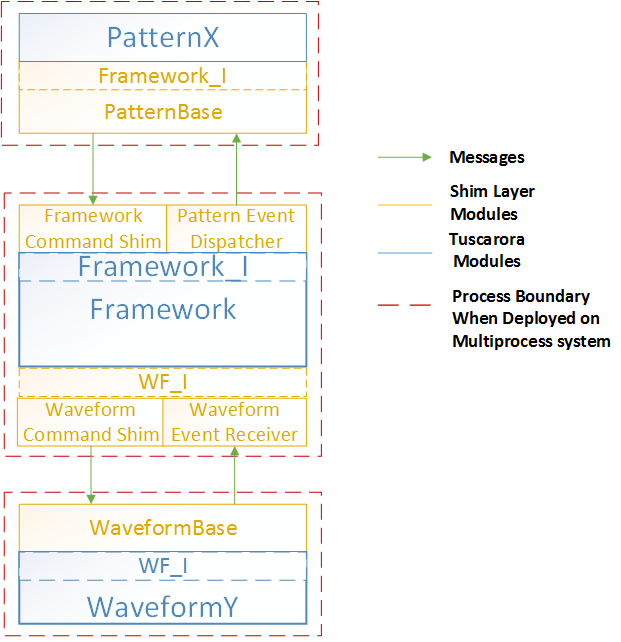
\includegraphics[width=0.7\linewidth]{figures/ShimArchitecture}
%	\caption{Pattern-Framework-Waveform interface}
%	\label{fig:ShimLayerInterface}
%\end{figure}

\begin{figure}[ht]
\centering
	  \begin{minipage}[b]{0.6\textwidth}
	    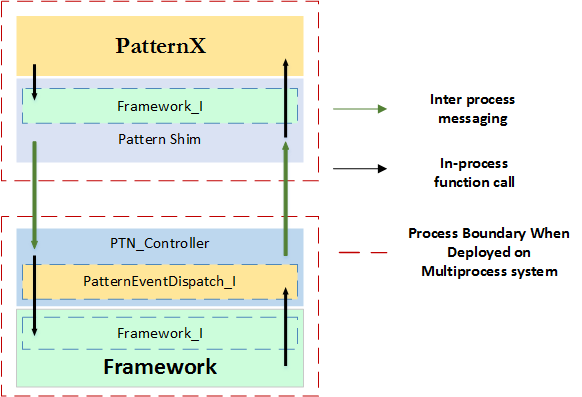
\includegraphics[width=\textwidth]{figures/Pattern_Framework_ShimArchitectureMP}
	    %\caption{multi process platform}
	    %\label{fig:PatternFrameworkInterface-MP}
	  \end{minipage}
%	  \hspace{3mm}
	  \begin{minipage}[b]{0.6\textwidth}
	    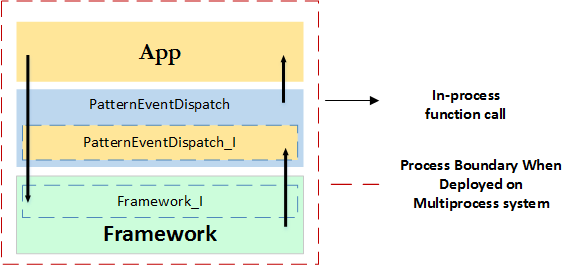
\includegraphics[width=\textwidth]{figures/Pattern_Framework_ShimArchitectureSP}
	    %\caption{single process platform}
		%\label{fig:PatternFrameworkInterface-SP}
	  \end{minipage}
\caption{Pattern-Framework interface for multi process and single process environments}
\label{fig:PatternFrameworkInterface}
\end{figure}

In order to facilitate the Pattern development, Tuscarora package comes with a common base class library, namely \CPPClassName{PatternBase}, that automates connections in the Pattern-Framework interface. For patterns deriving from it,  \CPPClassName{PatternBase} choses the shim classes required by the platform, initiates the communication medium with the Framework and provides patterns an abstracted pointer to the Framework through a member variable called \CPPVarName{FRAMEWORK}. Thus, for convenience Patterns are expected to inherit from \CPPClassName{PatternBase}, although it is not strictly necessary, 

The implementation of \CPPClassName{PatternShim} is platform-specific since implementing the Framework\_I interface to communicate with the actual framework will depend on the types of communication mechanisms available on a given platform. PatternBase also receive the \CPPClassName{Framework\_I} Events and convert them back into delegate calls for the Patterns. The corresponding Shim layer on the framework side is implemented by two classes-- one for Commands by the \CPPClassName{FrameworkShim} and one for Events by the \CPPClassName{PatternEventDispatch}. \Cref{fig:PatternFrameworkInterface} shows the flow of messages and bindings for this scenario..

In the DCE, the shim layers are implemented using synchronous function calls, since they are part of the same process space as shown in \cref{fig:PatternFrameworkInterface}. PatternBase gets a pointer directly to the FrameworkShim class (which is the shim class on the framework side) and invokes commands on it. Similarly the PatternEventDispatch module gets access to the Delegate objects in PatternBase and directly invoke them to implement the Events. 
 
\section{Framework-Waveform Shim Layer Modules} \label{sec:WaveformFrameworkInterface}
 
For the shim layer between the Framework and Waveform, the \CPPClassName{WF\_Controller} implements the commands in the WF\_I interface and ``Waveform Event Receiver'' module implements Events in WF\_I interface. 

On the waveform side the commands are directly provided by the modules that implement the WF\_I (i.e no shim in the forward direction in necessary) and the Events part of the WaveformBase shim are implemented \CPPClassName{AsyncEvent\_Special} module.

Once again, since in DCE we are in a single process address space, the shim modules directly get access to the objects on the other side and invoke them. The multi process and single process case interfaces are depicted in \cref{fig:FrameworkWFInterface}.

\begin{figure}[ht]
\centering
	  \begin{minipage}[b]{0.4\textwidth}
	    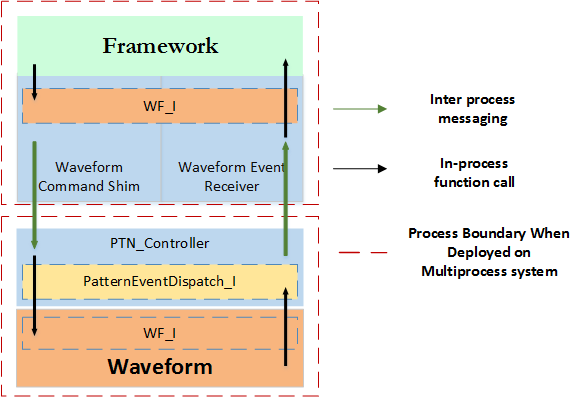
\includegraphics[width=\textwidth]{figures/Framework_Waveform_ShimArchitectureMP}
%	    \caption{multi process platform}
	%    \label{fig:FrameworkWFInterface-MP}
	  \end{minipage}
	  \hspace{5mm}
	  \begin{minipage}[b]{0.4\textwidth}
	    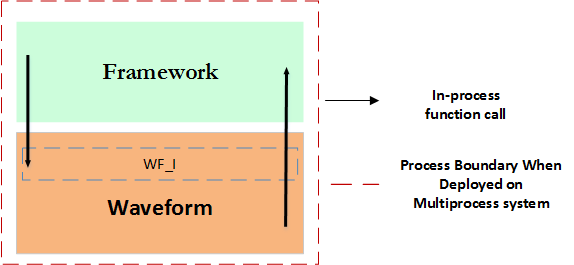
\includegraphics[width=\textwidth]{figures/Framework_Waveform_ShimArchitectureSP}
	    %\caption{single process platform}
		%\label{fig:FrameworkWFInterface-SP}
	  \end{minipage}
\caption{Framework-Waveform interface for multi process and single process environments}
\label{fig:FrameworkWFInterface}
\end{figure}


\iffalse 
The interface controlling messaging from the \TuscConcept{Framework} to the \TuscConcept{waveforms} is declared in \CPPClassName{Waveform\_I}. The framework keeps a pointer to this interface and simply invokes the functions declared in \CPPClassName{Waveform\_I}.

The messaging from the \TuscConcept{waveforms} to the \TuscConcept{Framework} is handled by the declarations provided by the templated class \CPPClassName{WF\_Event}. 
\CPPClassName{Waveform\_I} declares separate event types for various events such as 
\begin{itemize}
\item received message event (\CPPClassName{WF\_RcvMessageEvent\_t}), 
\item data notification event (\CPPClassName{WF\_DataNotifierEvent\_t}), 
\item link estimation event (\CPPClassName{WF\_LinkEstimateEvent\_t}),   %(WF_LinkEstimateEvent_t)
\item control response events (\CPPClassName{WF\_ControlResponseEvent\_t}), and
\item schedule update event (\CPPClassName{WF\_ScheduleUpdateEvent\_t}).
\end{itemize}
The waveform creates an event object of the corresponding type and a parameter object that is initialized with the information that is being transferred to the \TuscConcept{Framework}. 
Once the parameter is initialized, the waveform can simply invoke the event with the parameter. 
The event class the information using the shim layer to the Framework,
where it will be routed to the particular module that will process the received waveform data message. 
\fi


%/**
%  # Received Message Event #
% ## Invoke Method Definition ##
% * bool WF_RcvMessageEvent_t::Invoke (WF_RecvMsgParam param);
% * 
% * The Received Message Event class has a single public method called Invoke, which can be use do send the event to the framework, with WF\_RecvMsgParam as
% * the parameter.
% ## Expected Behavior: ##
% * When the waveform receives a valid data message through its radio interface, the waveform should event the Framework using the ``Receive Message Event''.
% * Upon receipt of a message, waveform will evaluate metadata (RSSI, SINR, Receive Timestamp) associated with the message and the metadata will be added to
% * the packet structure and passed in the parameter to the event.
% * An operating mode wherein the waveform forwards up to the Framework each and every packets that it receives and decodes correctly irrespective of whether
% * the packet was destined for the node is commonly referred to as ``promiscuous mode''. The API does not take a position on whether or not waveforms should
% * support promiscuous mode. (Hence, no API is currently defined to configure such a mode). If a future programmatic decision is made to support promiscuous
% * mode of waveforms, a policy manager (through the Framework) will explicitly configure the waveform to operate in such a mode. Unless explicitly configured
% * a waveform should not send packets not intended for the node to the Framework.
% * Note to Pattern designers: If a waveform does send packets to the Framework that are not meant for a particular node, the Framework has no way of identifying
% * such packets. The Framework cannot guarantee to a Pattern that it will not receive such “unintentional” packets. If a Pattern does receive such packets they would have originated from the same Pattern instance on a neighboring node, but are not intended to be received on the current node (i.e., right pattern, wrong node). We recommend that Pattern designers consider the possibility of receiving some unintentional packets and make their patterns robust enough to handle them.
% ## Event creation and invocation: ##
% * The details of the WF_RecvMsgParam parameter, and the code for creation and invocation of the Received Message are shown below. The waveform provider
% * creates the event object and the parameter object. Further, it initializes the parameter object with the received data message, the rcvMsgId is assigned
% * a MessageId generated by the waveform for the messages received by it. Once the parameter is initialized, the waveform can simply invoke the event with the parameter. The event class will convert this into a message of the appropriate format and send it using the shim layer to the Framework,
% * where it will be routed to the particular module that will process the received waveform data message.
% 
% #  Data Notification Event #
% ## Invoke Method Definition ##
% * bool WF_DataNotifierEvent_t::Invoke (WF_DataNotifierParam param);
% * The Data Notification class has a single public method called Invoke, which can be use do send the event to the framework, with WF_DataNotifierParam as
% * the parameter.
% ## Expected Behavior:
% * When a ‘SendData’ or ‘BroadcastData’ command is received by the Waveform, the Framework expects a Data Notification Event in response. The ackType in the parameter of the Data Notification Event indicates the type of notification. For each SendData command received with a particular MessageId, the waveform should send back at least two events, one of the ACK_WF_RECV type, indicating that the waveform received the message successfully and one of the ACK_WF_SENT type, indicating the waveform sent the message out through its radio. A third type named ACK_DST_RECV can also be sent if the waveform supports acks from the destination. For the BroadcastData command, the first two types are required and the third is not required. The ‘dest’ field in the param is an array that determines for which destinations that notification is being sent. For example, if the Waveform chooses to send multiple physical messages corresponding to the same “MessageId” once for each destination, then a notification event can be sent once per destination or it can all be grouped together and sent as a single notification.
% ## Event Parameters:
% * The parameter creation and invocation is quite similar to that of the other events. The waveform needs to create an object of WF_DataNotifierEvent_t,
% * create an object of the WF_DataNotifierParam and invoke the event with the param. The parameter for this event is show below.
% 
% # Link Estimation Event
% ## Invoke Method Definition
% * bool WF_LinkEstimateEvent_t::Invoke (WF_LinkEstimateParam param);
% * The Link Estimation Event class has a single public method called Invoke, which can be use do send the event to the framework, with WF_LinkEstimateParam as the parameter.
% ## Expected Behavior:
% * Link estimation of known neighbors is an optional function that the waveforms can choose to provide. If supported, the waveform should set the ‘estType’ field in its Attribute to WF_EST_FULL whenever it responds to the AttributeRequest.
% * Waveform that provide link estimation should provide link estimation events, and follow a standard format. The Framework defines a link metric structure that the waveform should compute for each neighbor. The WF\_LinkMetrics structure is show below, it consist of four metrics that are defined as follows:
% * 1. Quality: Abstract quality metric expressed as a real number between [0,1].
% * 2. Data rate: Link data rate expressed as log_2(bps).
% * 3. Average Latency: Average latency in sending a packet to the destination expressed as log_2(seconds).
% * 4. Energy: Average energy to transmit a packet expressed as log_2(pica-joules).
% * 
% The waveform is expected to generate a event for each neighbor whenever one of the three events happens:
% * 1. New Neighbor: Whenever the waveform detects a new neighbor and has an initial estimate of its link metrics. It uses the value NBR_NEW for the ‘changeType’ field of the event parameter.
% * 2. Dead Neighbor: Whenever a previous neighbor no longer exist in the neighbor. Use the value NBR_DEAD for the ‘changeType’ field of the event parameter
% * 3. Change in Metrics: Whenever the metrics has changed enough to notify the Framework. It uses the value NBR_UPDATE for the ‘changeType’ field of the event parameter.
% ## Event Parameters:
% * The  WF_LinkEstimateParam structure (shown above) is used as the parameter for the Link Estimation Event. The structure contains the waveform address, the link type, its link metrics and the type of change in neighborhood being conveyed by the message.
% # Control Response Event
% ## Invoke Method Definition
% * bool WF_ControlResponseEvent_t::Invoke (WF_ControlResponseParam param);
% * The Control Response Event class has a single public method called Invoke, which can be use do send the event to the framework, with WF_ControlResponseParam as the parameter.
% ## Expected Behavior:
% * Whenever a waveform receives any request command, i.e., a command whose name has the suffix Request, it should use the Control Response Event to send a response. The response should use the same “RequestId” as in the request command. The Framework tracks the RequestId that it uses for each waveform and generates a new RequestId for every request command. If the Framework fails to receive a response for a request, the Framework may resend the request using the same RequestId.
% ## Event Parameters:
% * The WF_ControlResponseParam parameter associated with the Control Response is shown below. The key field is ‘type’, which is an enum of type WF_ControlResponseE. This enumerator defines a response for each of the Request commands. The waveform should set this type appropriately based on the command it is responding too. The parameter also contains a generic ‘data’ field, whose interpretation by the Framework depends upon on the type of the response. Based on the type of Request command that is being responded to, an appropriate structure is copied into the ‘data’ field, and the number of bytes sent through the data field should be set appropriately in the dataSize  field.
% 
% # Schedule Update Event
% ## Invoke Method Definition
% * bool WF_ScheduleUpdateEvent_t::Invoke (WF_ScheduleUpdateParam param);
% * The Schedule Update Event class has a single public method called Invoke, which can be use do send the event to the framework, with WF_ScheduleUpdateParam as the parameter.
% ## Expected Behavior:
% * Schedule updates are an optional feature by which waveforms that maintain schedules for functions such as sending, receiving or link estimation can share information about the schedules with the Framework. If the feature is supported, the waveform should set as true the ‘schedulerInfoSupport’ field in its Attribute whenever it responds to the AttributeRequest.
% * This event is expected to be implemented by waveforms that have timing characteristics or TDMA schedules. The eventing should be implemented if the knowledge of a waveform's slot schedules will help the Framework in improving the overall data efficiency.
% * Note: If the waveform is responding to the ‘ScheduleRequest’ command, then it should use the Control Response Event; and, if it is sending ongoing schedule updates, it should use the Schedule Updates Event.
% ## Event Parameter
% * The WF_ScheduleUpdateParam structure that is used as the parameter of the Schedule Update Event is shown below. The parameter contains information about one of three types of schedules,  send, receive or link estimation, which is indicated by setting the ‘type’ field appropriately. The ‘data’ field is a pointer of type ScheduleBaseI which points to the object that contains the actual schedule information for the neighbor indicated by ‘nodeid’. 
% * The dataSize field contains the size of the actual schedule object that is pointed to by the data field.
% */
% 



\section{NS3-DCE}

For portability reasons, this release uses the Direct Code Execution (DCE)~\cite{dce} environment for running simulations. 
DCE is a module that enables ns-3 simulator to run existing source code that is targeted towards POSIX environments. 
%In short, DCE lets users develop code that can be directly deployed on POSIX systems or run them in simulation. 
The executable for each node runs on a separate process and these processes are coordinated through another process running ns3 simulator.  
%\section{Message Passing Interfaces}
For more information see the DCE documentation~\cite{dce}.


